\newpage % Zaleca się otwieranie rozdziału od nowej strony.
\section{Dobór komponentów i projektowanie konstrukcji mechanicznej}


\subsection{Założenia projektowe}
Do realizacji zamierzonych celów niezbędne będzie dobór komponentów, czyli mikrokontrolera wykonującego wszystkie obliczenia i sterowania, silników sterujących długością nóg, joysticka zadającego pozycję, panelu dotykowego, a także zaprojektowanie i wykonanie konstrukcji mechanicznej. 
Całość potem trzeba połączyć i odpowiednio zaprogramować. Projektując urządzenie wybierałem przede wszystkim sprawdzone, ale też niedrogie komponenty. 

\subsection{Mikrokontroler}
Sterowanie sześcioma nogami wymaga sześciu wyjść PWM. 
Z kolei do odczytywania położenia kulki przez panel dotykowy i zadawanego przez joystick potrzebne są cztery wejścia ADC o wysokiej rozdzielczości. 
Dodatkowo złożoność obliczeniowa algorytmów sterujących i obliczających długość nóg powoduje, że najlepiej sprawowałby się szybki mikrokontroler z jednostką FPU. 
Okazuje się, że wystarcza mikrokontroler z częstotliwością taktowania 64 MHz bez FPU, którego obecność znacznie przyśpieszyłaby wykonywanie obliczeń na liczbach zmiennoprzecinkowych.
Zdecydowałem się na 32-bitowy mikrokontroler z rodziny ARM z rdzeniem Cortex-M3 od firmy STMicroelectronics - STM32f103rb6. Ułatwiony dostęp do programowania zapewnia płytka ewaluacyjna NUCLEO-F103RB.


\begin{figure}[!h]
    \label{fig:anzelm}
    \centering
    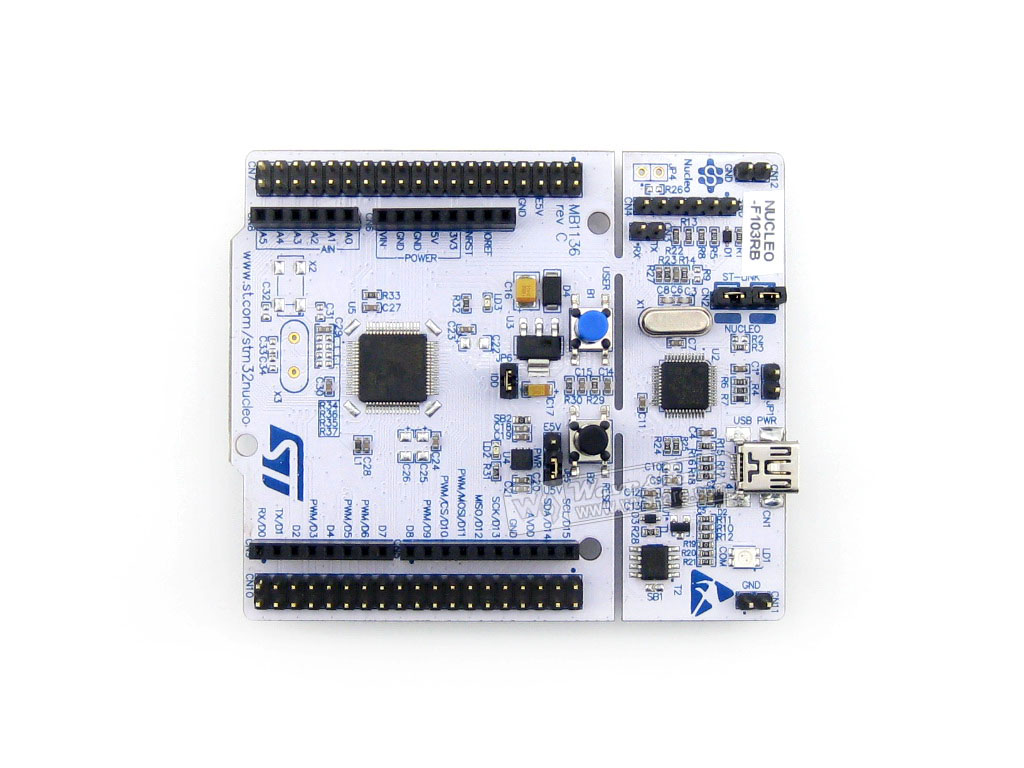
\includegraphics[width=0.5\linewidth]{img/NUCLEO-F103RB-5.jpg}
    \caption{Płytka ewaluacyjna NUCLEO-F103RB od firmy STMicroelectronics.}
    % \captionsource{Źródło: }{https://www.st.com/en/evaluation-tools/nucleo-f103rb.html}
\end{figure}

Taka płytka oferuje 12-bitowe przetworniki ADC, zegar główny taktujący z częstotliwością 64 MHz, a zasilania jest niskim napięciem od 2 do 3.6V. Niskie napięcie zasilania i architektura ARM (Advanced RISC Machine) sprawiają, mikrokontroler będzie pobierac niewiele mocy.


\subsection{Jak wykonać nogi? Dlaczego serwo? Dobór przegubów}
Ze względu na wysoki koszt liniowych aktuatorów, długość nóg będzie zmieniania poprzez zmianę wychylenia serwomechanizmów z przymocowanymi prętami. Zestaw złożony z serwomechanizmu, ramienia i pręta zakończonego dwoma przegubami kulkowymi stanowi jedno odnóże i pełni rolę pary kinematycznej.

\begin{figure}[!h]
    \label{fig:anzelm}
    \centering
    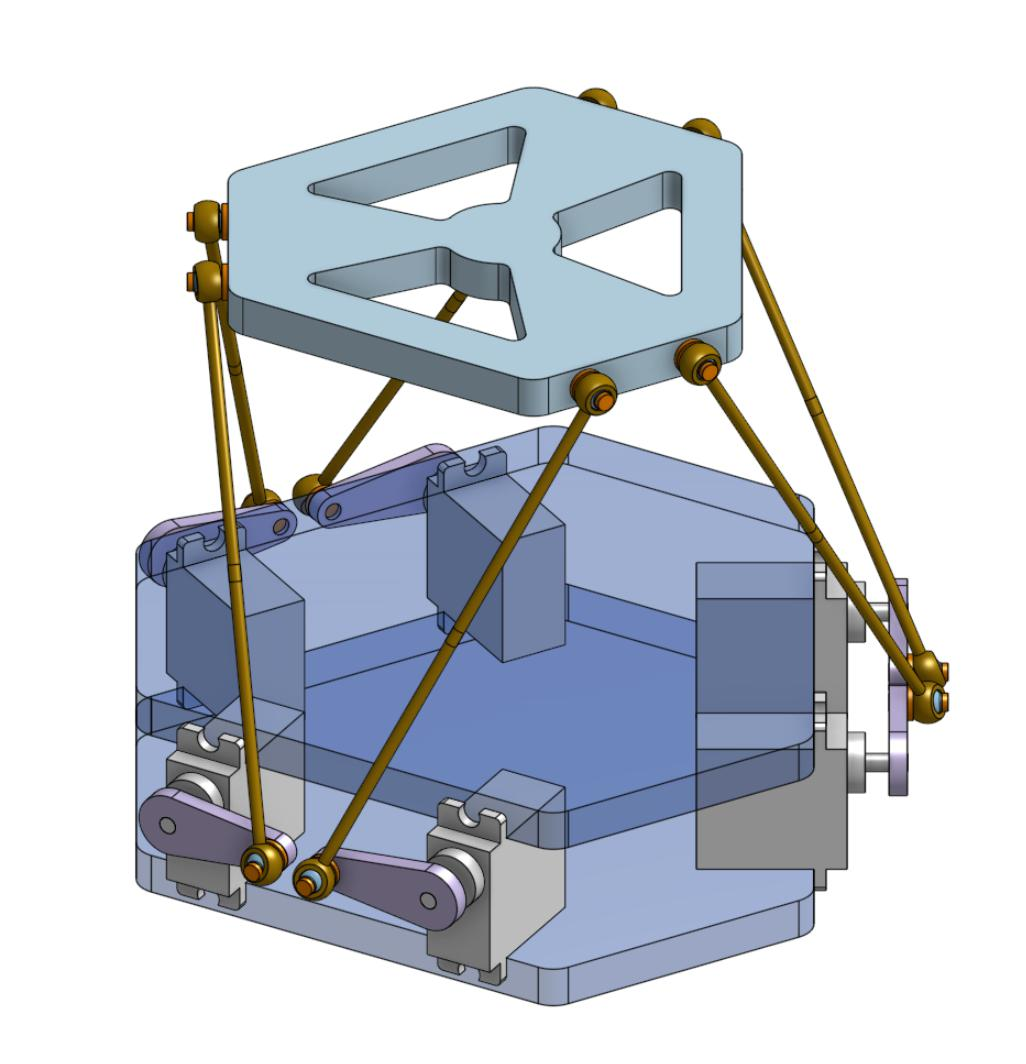
\includegraphics[width=0.5\linewidth]{img/stewart_servo_github.jpg}
    \caption{Projekt platformy Stewarta z wykorzystaniem serwomechanizmów.}
    % \captionsource{Źródło: }{https://ouilogique.com/plateforme-de-stewart-esp32/}
\end{figure}


W celu zapewnienia pełnego zakresu ruchów takiej parze kinematycznej, potrzebne jest skorzystanie z odpowiednich przegubów. Wykorzystałem przeguby z trzema rotacyjnymi stopniami swobody, znanymi w modelarstwie pod nazwą ,,snap kulowy``.

\begin{figure}[!h]
    \label{fig:anzelm}
    \centering
    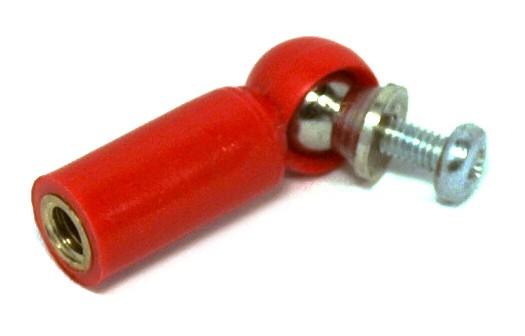
\includegraphics[width=0.5\linewidth]{img/snap_kulowy.jpg}
    \caption{Snap kulowy, albo lepiej przyklad nogi.}
    % \captionsource{Źródło: }{https://ouilogique.com/plateforme-de-stewart-esp32/}
\end{figure}

\subsection{Wybór serwomechanizmu}
Rezygnując z aktuatorów liniowych na rzecz serwomechanizmów znacznie zmniejszyłem koszty projektu, licząc się jednak ze zmniejszeniem siły nośnej platformy.
Szukając odpowiednich serw, zauważyć można zależność, że wraz z większym momentem siły generowanym na wale serwa, rosną jego wymiary i cena.
W przypadku platformy Stewarta, ciężar górnego talerza, panelu dotykowego i kulki jest rozkładany na wszystkie nogi, co nie kładzie dużych wymagań udźwigowych na jeden silnik.
Jednak by zwiększyć zakres wychyleń talerza górnego trzeba zapewnić odpowiednią długość ramienia.
Chcąc uzyskać zmianę długości nogi w zakresie 60-70 mm, takie ramie powinno mieć 35 mm długości. 
\\ \\
W takim razie, jak dobrać odpowiedni serwomechanizm? \\
Cały górny talerz z kulką będzie ważyć 600 g, czyli jedna noga powinna udzwignąć minimum 100 g, a ramie serwa będzie wynosić 35 mm.
Producenci serw podają jako parametr moment siły wału obracającego się w jednostkach [kg*cm].
Przekształcając wzór na moment siły (T) i podając długość ramienia (r) można obliczyć z jaką siłą maksymalnie może udzwignąć jedna noga platformy, przy założeniu, że wektory siły F i wektor promienia wodzącego r skierowane są względem siebie pod kątem prostym.
\begin{equation}
    \vec{T} = \vec{F} * \vec{r}
\end{equation}{}
\begin{equation}
    F_{max} = \frac{T_{max}}{r_{orczyk}}
\end{equation}{}

Podstawiając do wzoru na siłę stałą grawitacyjną ($g=9.81 [m/s^2]$) można obliczyć maksymalny udźwig platformy z 6 silnikami.
Należy pamiętać, że jest udźwig przy maksymalnym poborze prądu serwomechanizmu i z prostopadłym ułożeniem prętu nogi względem ramienia serwa. 
Zakładając realne warunki pracy można szacować, że w rzeczywistości będzie to zaledwie 70-80 \% obliczonej wartości.

% Wrzucicc tabelke z porównaniem różnych serw - opisac jaki byłby maxymalny moment i ze te 3kg z obliczen by bylo ok
\begin{table}[!h]
\begin{tabular}{|l|l|l|l|l|l|}
\hline
Nazwa mechanizmu & $T_{max} {[}Nm{]}$ & $F_{max_{6 sztuk}} {[}N{]}$ & napięcie zasilania ${[}V{]}$ & $m_{critical} {[}kg{]}$ & Cena za sztukę {[}zł{]} \\ \hline
TowerPro SG-90 & 0,18 & 30,24 & 4,5 - 6 & 3,09 & 8 \\ \hline
TowerPro SG-92 & 0,24 & 42 & 4,5-6 & 4,29 & 15 \\ \hline
PowerHD HD-1160A & 0,27 & 45,36 & 4,5-6 & 4,63 & 19 \\ \hline
\end{tabular}
% W jaki sposob ma to trafic do spisu tabel?
\end{table}

Zdecydowałem się więc na bardzo popularny i tani serwomechanizm SG-90 z zakresem ruchu wynoszącym 180 stopni, co jak najbardziej wystarcza do zmiany efektywnej długości nogi, a jednocześnie oferuje wystarczającą moc mechaniczną. \\\\
 Jednak praca z tymi silnikami okazała się uciążliwa ze względu na układ przekładni, który został wykonany z plastiku i niestety często ulegał uszkodzeniom.
 Także na 6 wymaganych silników musiałem wykorzystać 9, ze względu na wyłamane zęby.
 Na szczęście niska cena serw pozwala lekko przymknąć oko na jakość wykonania. 
 \\
 Producent także podaje, że pobór prądu przez jedno serwo wynosi od 100 do 700 mA przy zasilaniu 4,5 V w zależności od obciążenia.
 W takim wypadku 6 serw połączonych równolegle napięciem 4V będzie potrzebowało zasilania ok 3A, zakładając, że platforma nie będzie ciężka.
 

\subsection{Projekt konstrukcji}
Budowa mechaniczna platformy jest dosyć prosta, potrzebny jest sztywna dolna podstawa, na której znajdą się serwomechanizmy, połączona z górnym, też sztywnym talerzem za pomocą nóg. 
Na górnym talerzu znajdzie się panel dotykowy.
Mimo, że wykorzystanie technologii druku 3D nie jest niezbędne przy wykonywaniu takiego urządzenia, to jednak skorzystałem z takiej opcji i część elementów (podstawa do zamocowania serw, przedłużenie ramion serwomechanizmów, mocowanie nóg do górnego talerza) zaprojektowałem w programie Inventor od producenta Autodesk, a potem wydrukowałem.
\\
Ważne w konstrukcji jest odpowiednie rozmieszczenie serw na podstawie.
Popularnym rozwiązaniem jest budowanie podstawy na planie szesciokąta foremnego, lub okręgu. 
Zdecydowałem się na sześciokąt nieforemny, z serwami rozmieszczonymi na bazie okręgu, w taki sposób, ze każda para silników znalazła się na dłuższym boku sześciokąta i położona jest względem poprzedniej pary pod kątem 60 stopni.

Projektując rozkład serw chciałem, aby podstawa była odpowiednio dużo, żeby płytka ewaulacyjna z mikrokontrolerem spokojnie mogła być zamontowana na podstawie, a dostęp do pinów mikrokontrolera nie był ograniczony przez pokrywę.


\begin{figure}[!h]
    \label{fig:anzelm}
    \centering
    % Mozna poprawic, zeby zlapac ladniejszy kat platformy
    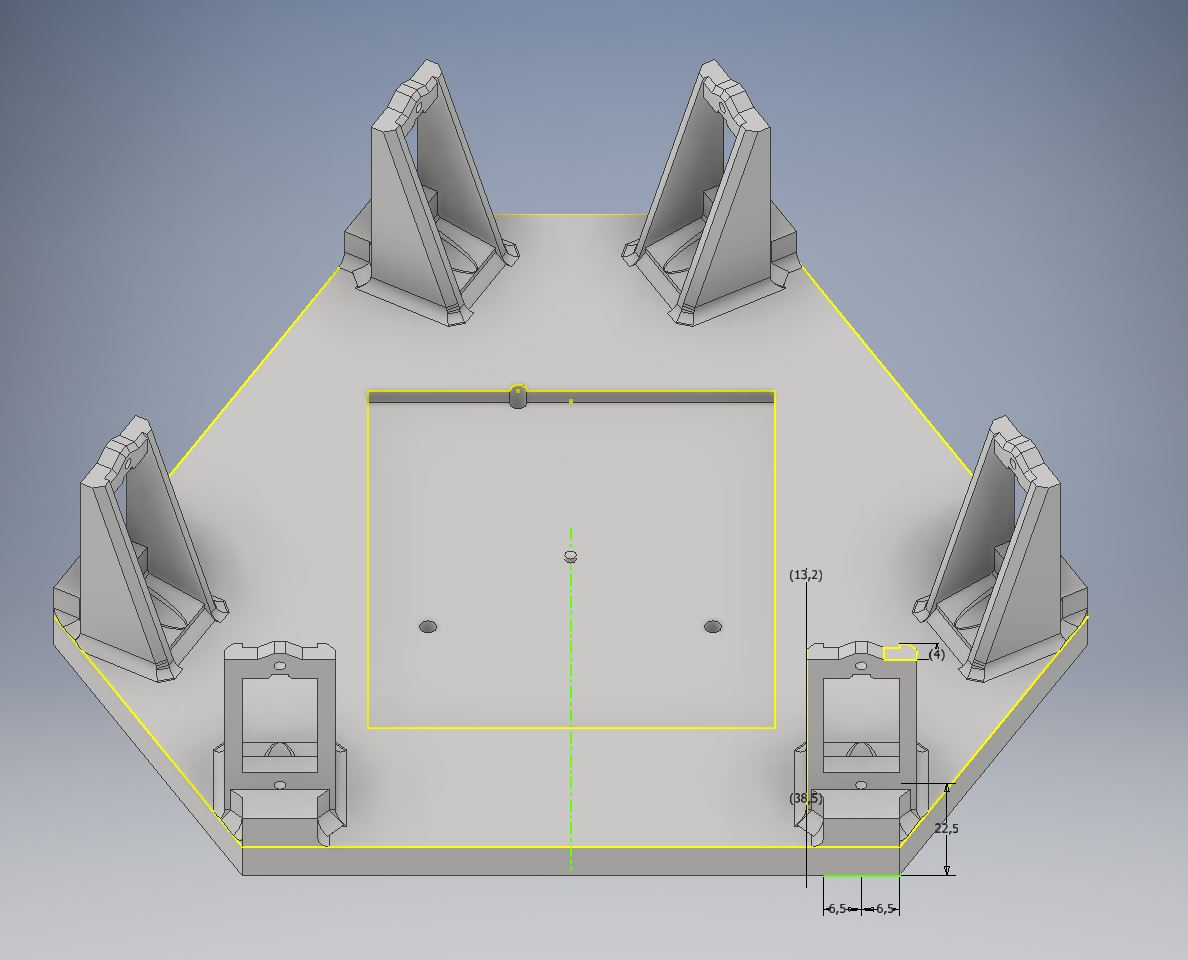
\includegraphics[width=0.5\linewidth]{img/Base_UP.JPG}
    \caption{Projekt platformy.}
    % \captionsource{Źródło: }{}
\end{figure}

Dodatkowo, kolejnym czynnikiem doboru wielkości platformy był porządany zakres ruchu talerza górnego.
Chcąc, by długość nogi zmieniała się w zakresie 35mm, trzeba było zapewnić odpowiedni dystans pomiędzy serwami.
Niestety orczyki, będące oryginalnie w zestawie serwomechanizmu są za krótkie.
Z tego też powodu niezbędne okazało się zaprojektowanie prostej nakładki przedłużającej oryginalny orczyk i wydrukowanie ich sześciu sztuk.

\begin{figure}[!h]
    \label{fig:anzelm}
    \centering
    % Trzeba dorzucic to co jest w opisie
    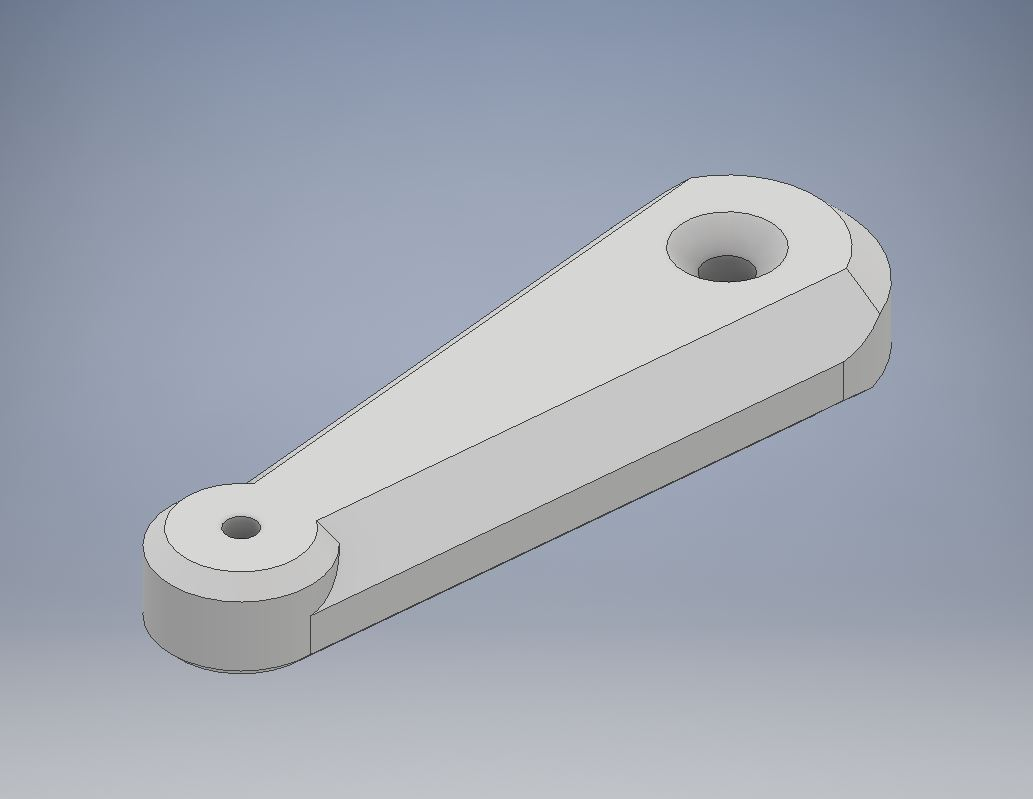
\includegraphics[width=0.5\linewidth]{img/serwo_orczyk_UP.JPG}
    \caption{Model 3D serwa, oryginalnego orczyka i zaprojektowanego przedłużenia.}
    % \captionsource{Źródło: }{}
\end{figure}
\begin{figure}[!h]
    \label{fig:anzelm}
    \centering
    % Trzeba dorzucic to co jest w opisie
    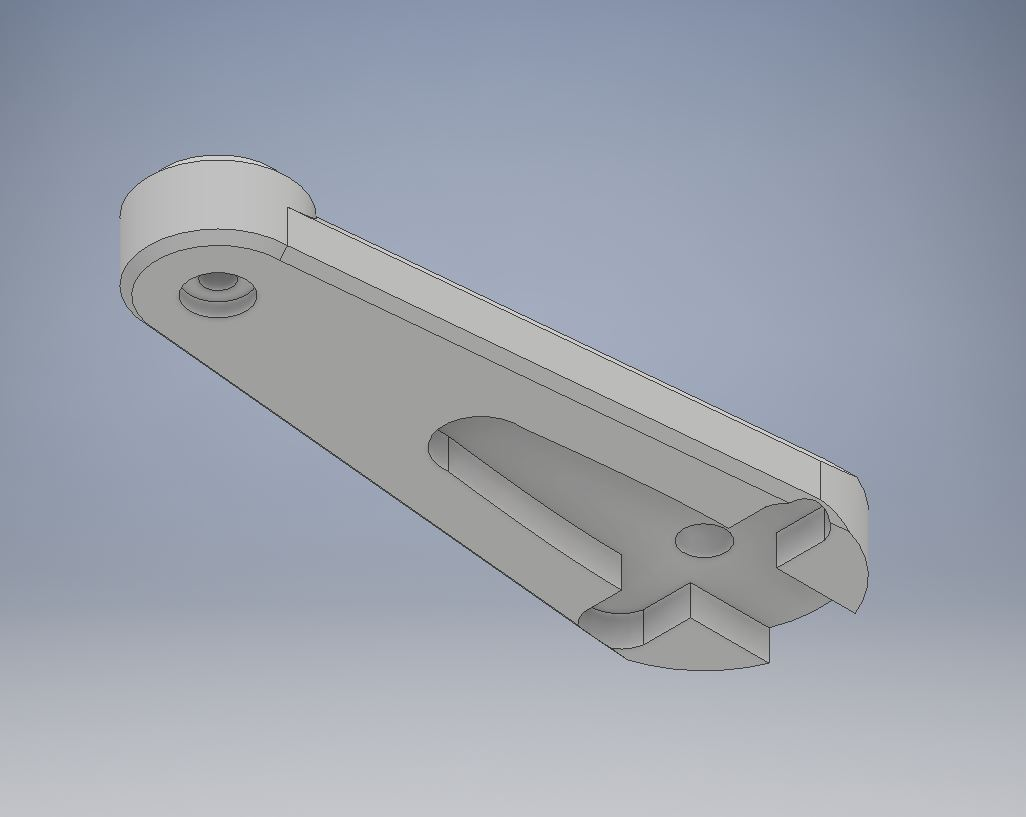
\includegraphics[width=0.5\linewidth]{img/serwo_orczyk_DOWNJPG.JPG}
    \caption{Model 3D serwa, oryginalnego orczyka i zaprojektowanego przedłużenia.}
    % \captionsource{Źródło: }{}
\end{figure}


\subsection{Panel dotykowy.}
Dobór panelu dotykowego był pozornie prosty. Na rynku można znaleźć panele dotykowe robione w dwóch technologiach - pojemnościowej i rezystancyjnej. 
Jako, że zasada działania i sposób odczytu położenia z panelu rezystancyjnego miał być prosty, wybór padł właśnie na ten typ.
Biorąc pod uwagę, że panel dotykowy pełni funkcję platformy, po której będzie poruszać się kulka, większa powierzchnia panelu jedyną porządaną cechą.
W pracy wykorzystuję więc panel rezystancyjny o przekątnej 7 cala, który komercyjnie dostępny jest jako panel dotykowy do nawigacji samochodowej.
Mikrokontroler może się z nim porozumieć za pomocą 4 przewodów w sposób analogowy, bez dodatkowych sterowników.

\begin{figure}[!h]
    \label{fig:anzelm}
    \centering
    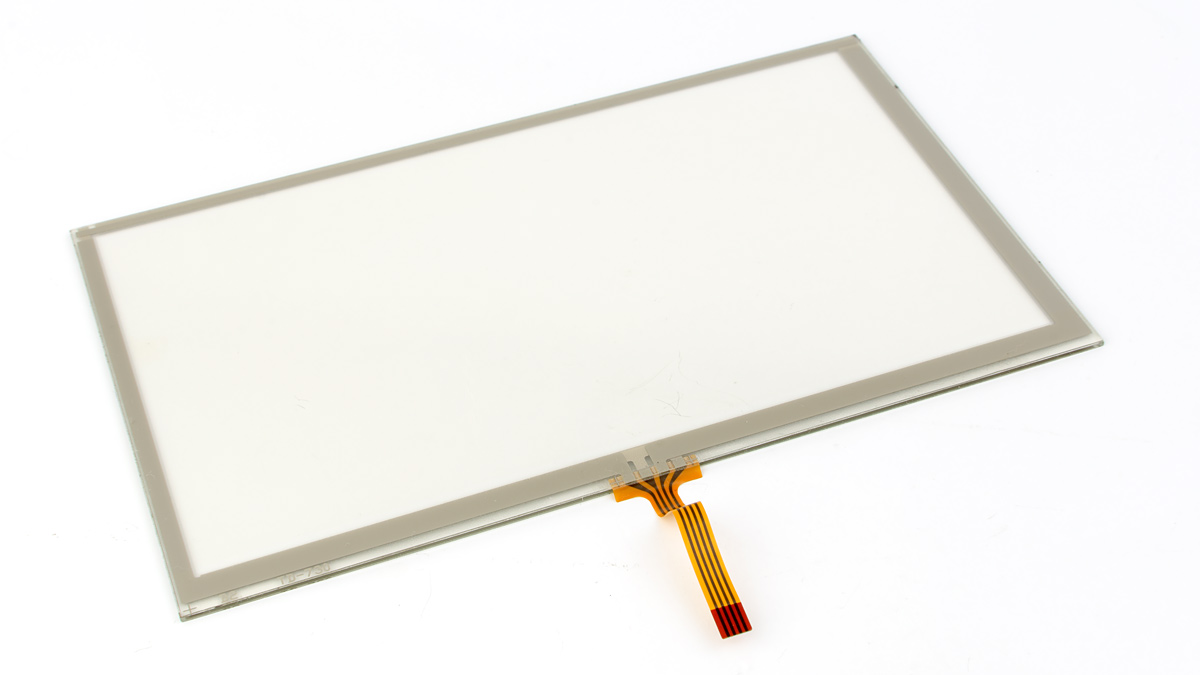
\includegraphics[width=0.5\linewidth]{img/resistive_7_inch_touchscreen_b.jpg}
    \caption{Rezystsancyjny panel dotykowy z dostępem 4-wire.}
    % \captionsource{Źródło: }{}
\end{figure}

Takie podejście okazało się czasochłonne i może lepiej było szukać wersji ze sterownikami i porozumiewać się za pomocą protokołu I2C.

\subsection{Kontroler zadawania położenia i orientacji.}
Żeby testować zadawanie konkretnego położenia platformie, wykonałem prosty kontroler. 
Do zadania zmiennych położenia w płaszczyźnie X, Y wykorzystałem joystick analogowy o maksymaknej rezystancji $4,7 k\Omega$, a do zmiany położenia osi Z potencjometr o rezystancji maksymalnej $10 k\Omega$.
Do odczytania kątów orientacji (Roll, Pitch i Yaw) kontrolera wykorzystałem czujnik IMU (Inertial Measurment Unit) LSM303D firmy Pololu z akcelerometrem i magnetometrem, który komunikuje się z mikrokontrolerem za pomocą protokołu I2C.

\begin{figure}[!h]
    \label{fig:anzelm}
    \centering
    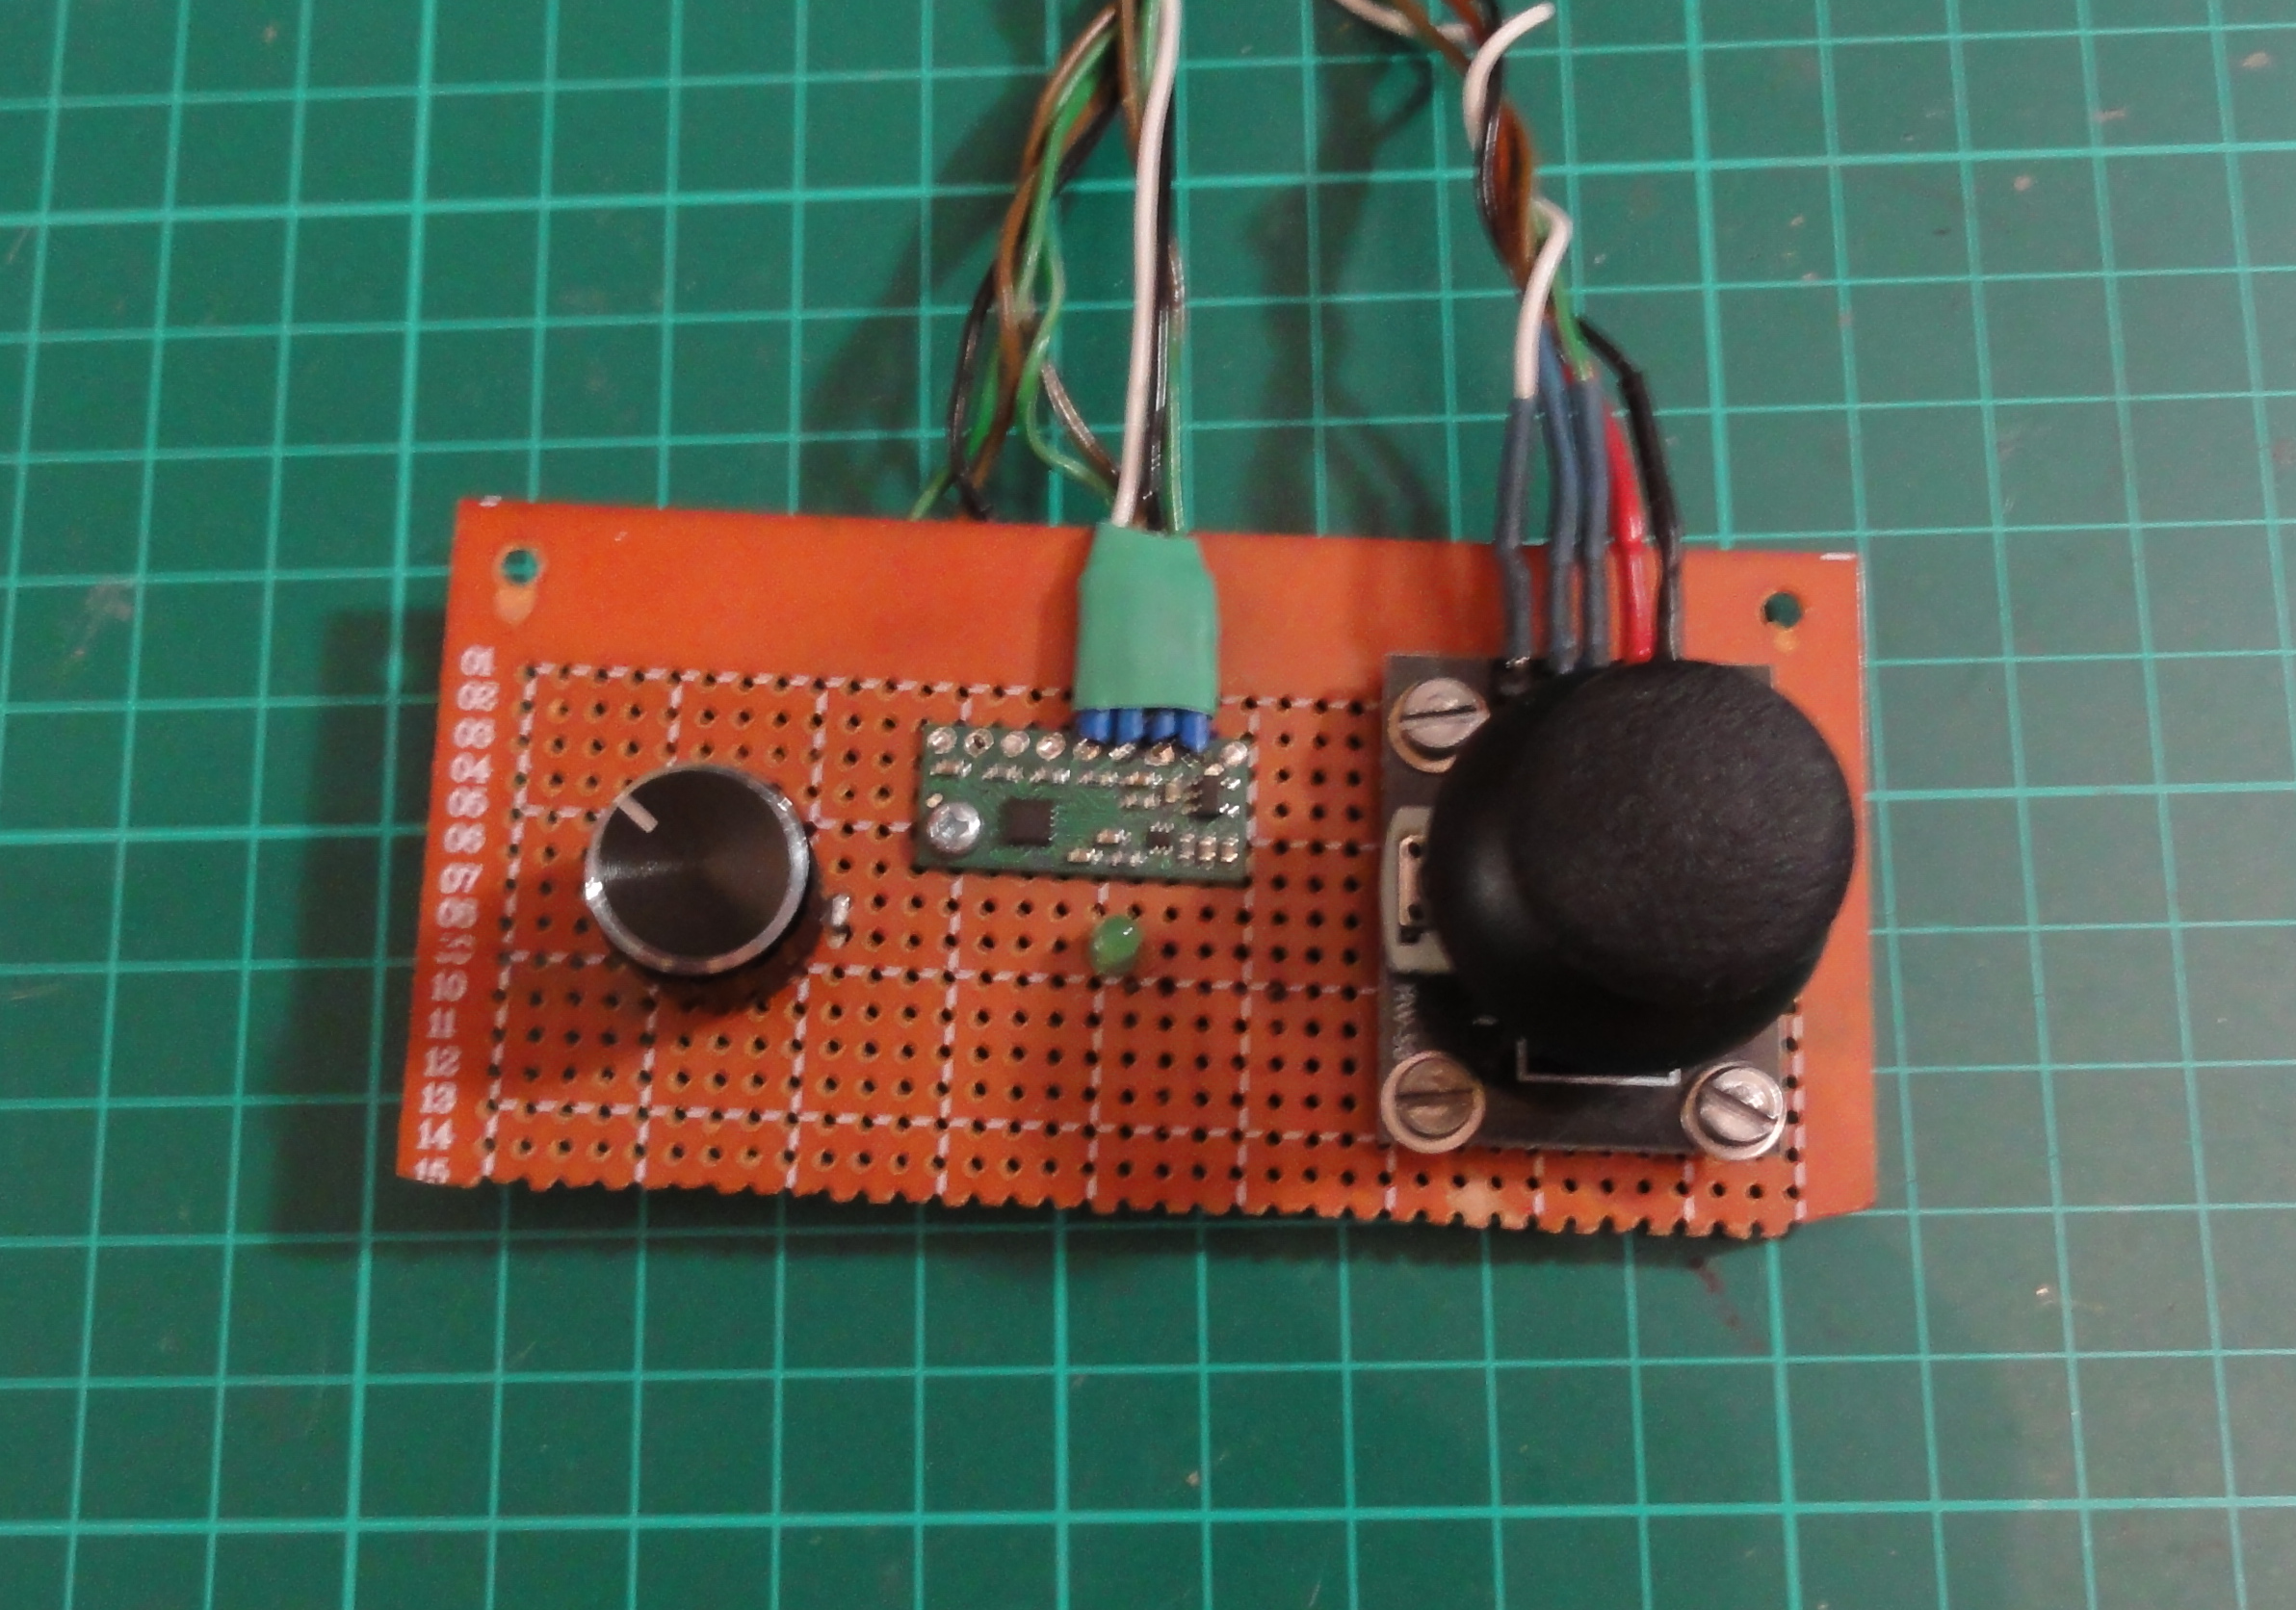
\includegraphics[width=0.3\linewidth]{img/kontroler_joystick_imu.jpg}
    \caption{Prosty kontroler zadawania pozycji platformie.}
    % \captionsource{Źródło: }{}
\end{figure}

\begin{figure}[!h]
    \label{fig:anzelm}
    \centering
    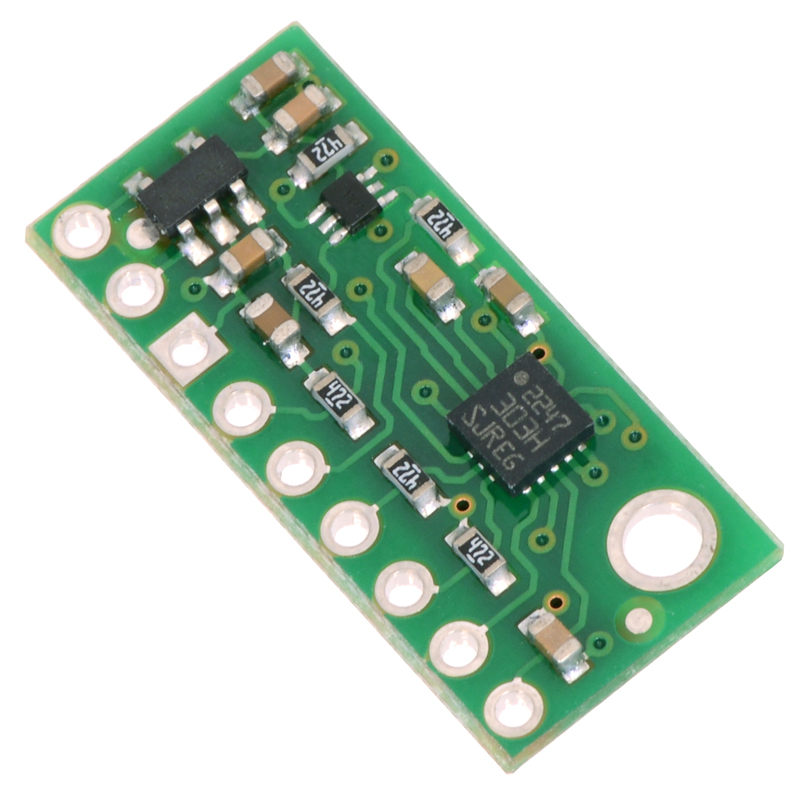
\includegraphics[width=0.3\linewidth]{img/Pololu_LSM303D.jpg}
    \caption{Płytka z mikroukładem elektromechanicznym (MEMS), zawierającym akcelerometr i magetometr.}
    % \captionsource{Źródło: }{}
\end{figure}



\subsection{Schemat elektryczny i zasilanie}
Fajnie pokazać zasilanie silników z ładowarki do telefonu, wybierając odpowiednie żyły kabla do USB.

\subsection{Łączenie elementów i finalna budowa.}

Mając wszystkie wydruki gotowe, wystarczyło zbudować całą platformę i podłączyć elementy elektroniczne.
Do przymocowania nóg do górnej platformy wydrukowałem dodatkowy element o kształcie podstawy, aby mieć pewność, że wymiary będą się zgadzać.
Do podstawy i górnego talerza, w celu zwiększenia masy i stabilności, a także aby orczyki serw nie uderzały o podłoże, dodałem warstwę z przyciętej płyty pleksi.
Dodatkowo, aby kulka nie spadała z talerza podczas doboru nastaw regulatora, przymocowałem do panelu barierkę wykonaną z balsy.

\begin{figure}[!h]
    \label{fig:anzelm}
    \centering
    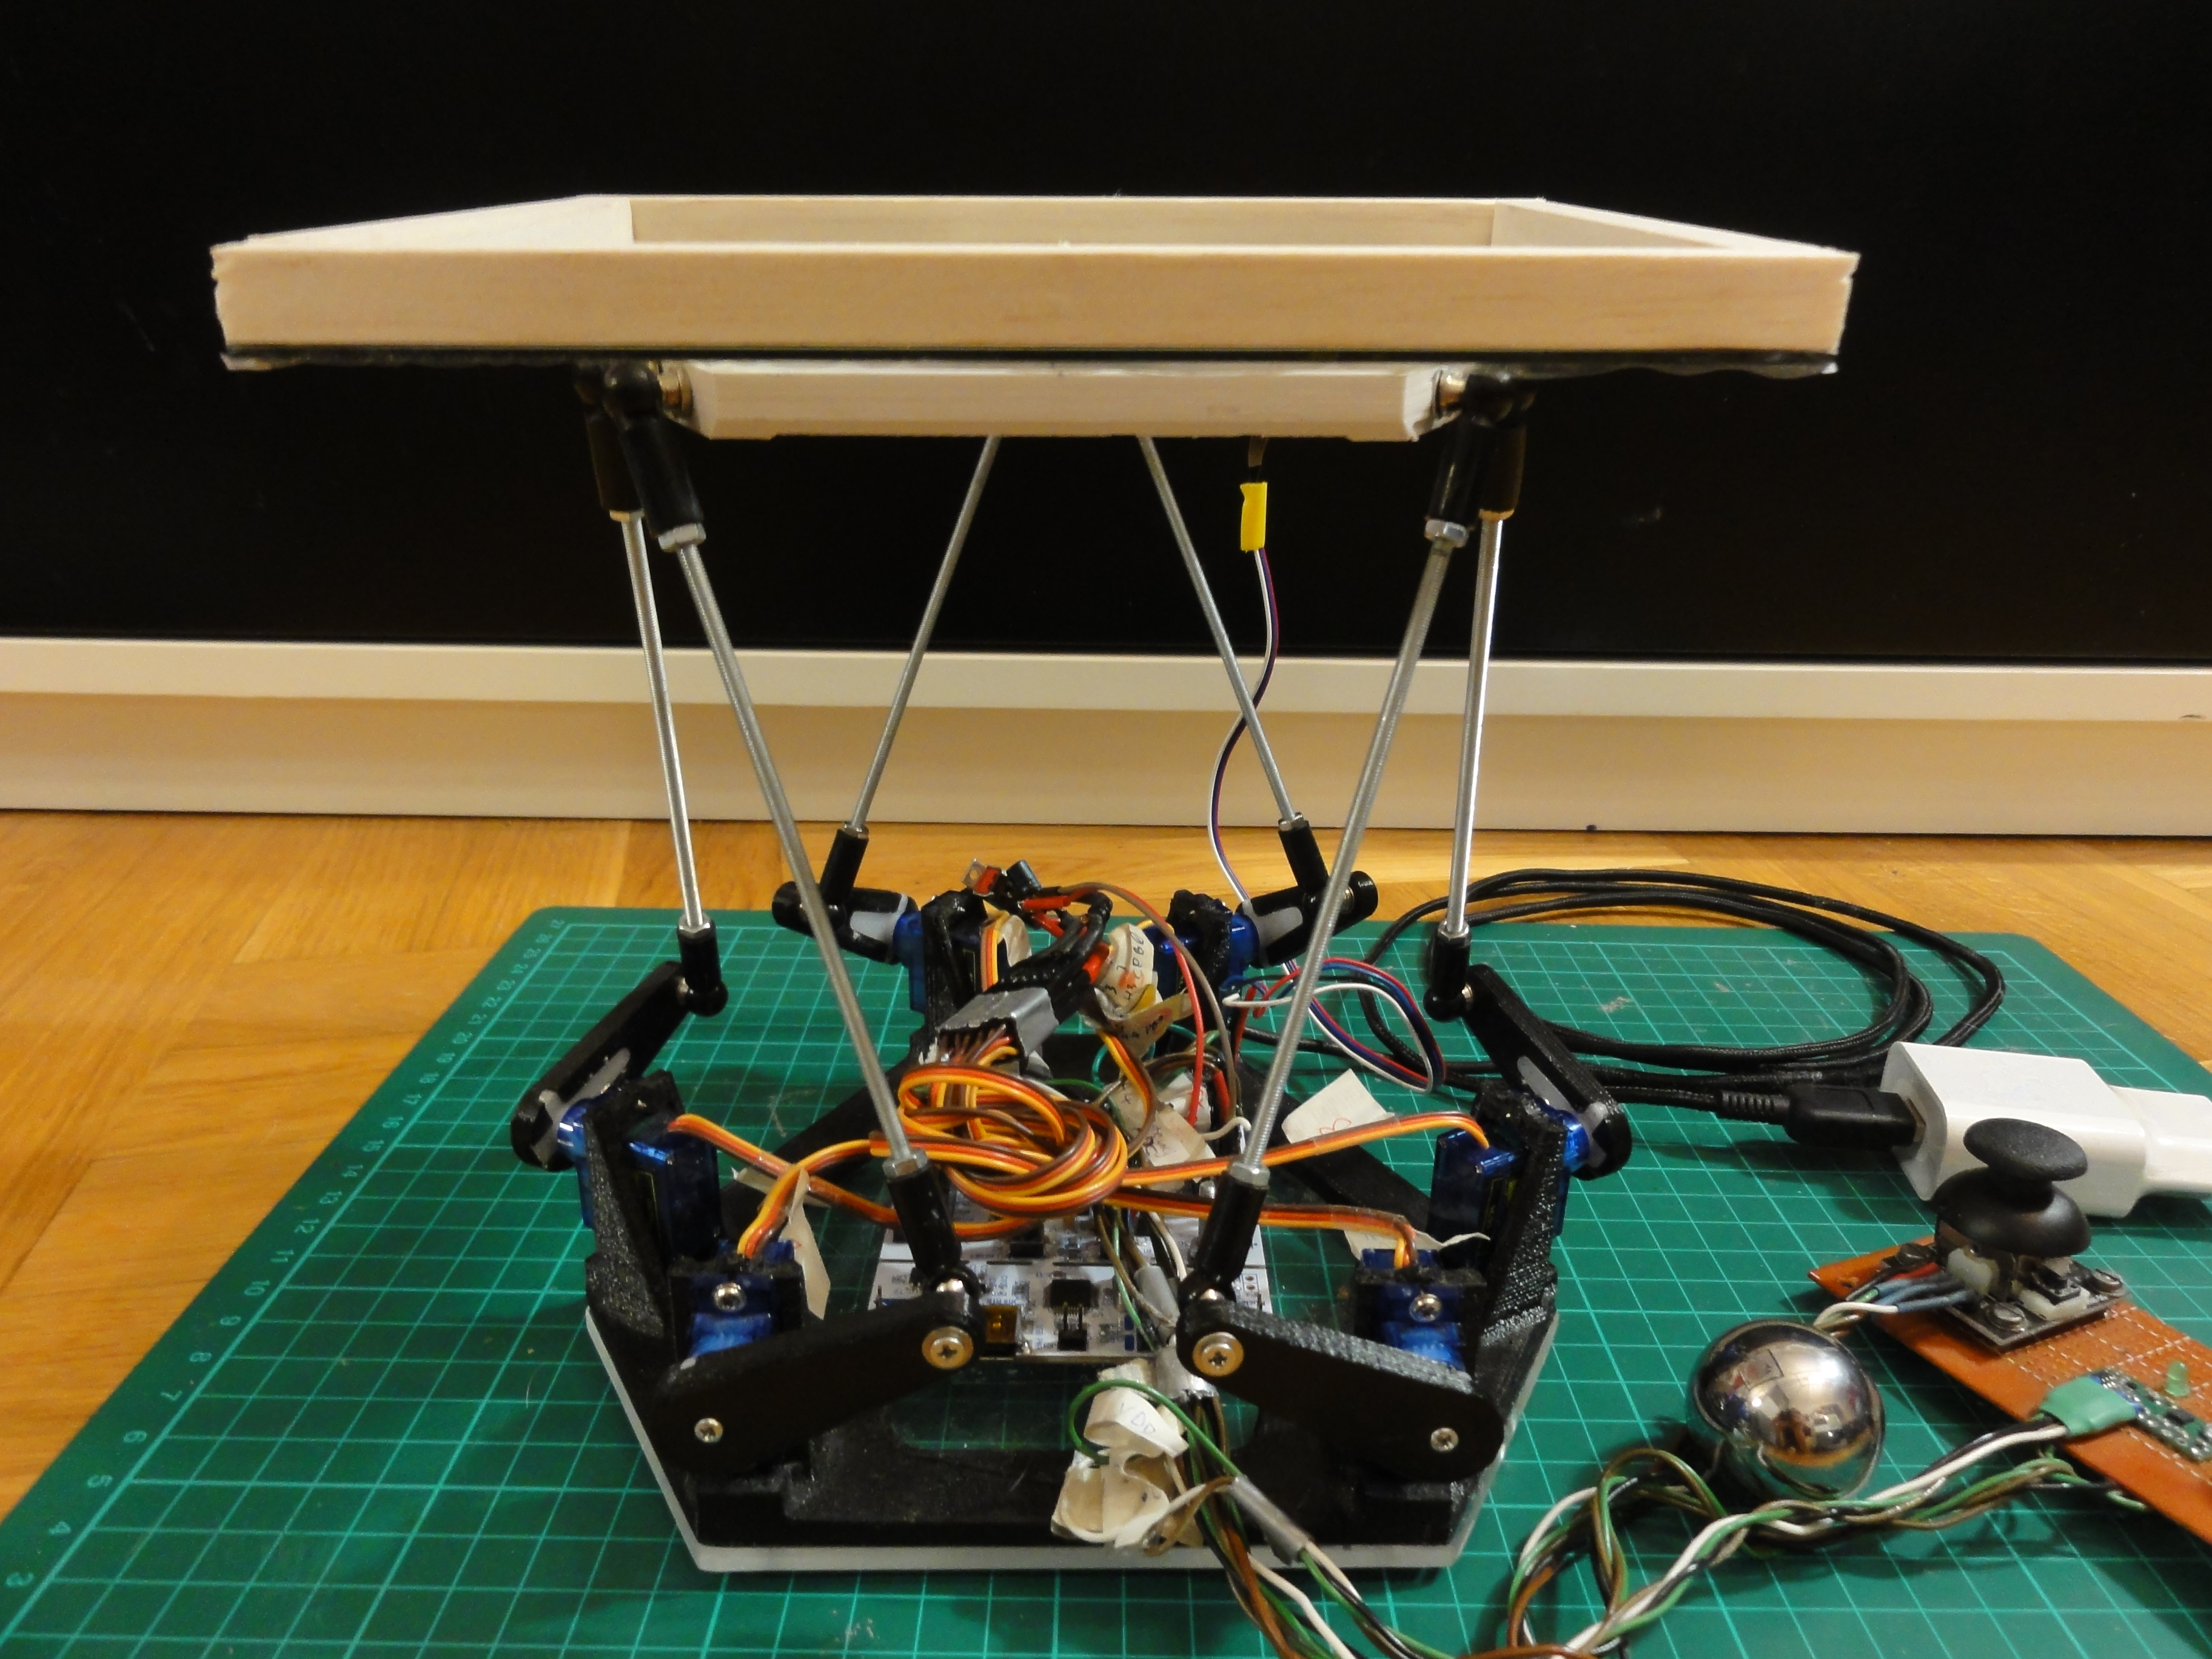
\includegraphics[width=0.5\linewidth]{img/Platforma_rzeczywista.JPG}
    \caption{Gotowa konstrukcja platformy wraz z kontrolerem, zasilaczem i kulką.}
    % \captionsource{Źródło: }{}
\end{figure}


